\PassOptionsToPackage{unicode=true}{hyperref} % options for packages loaded elsewhere
\PassOptionsToPackage{hyphens}{url}
%
\documentclass[]{article}
\usepackage{lmodern}
\usepackage{amssymb,amsmath}
\usepackage{ifxetex,ifluatex}
\usepackage{fixltx2e} % provides \textsubscript
\ifnum 0\ifxetex 1\fi\ifluatex 1\fi=0 % if pdftex
  \usepackage[T1]{fontenc}
  \usepackage[utf8]{inputenc}
  \usepackage{textcomp} % provides euro and other symbols
\else % if luatex or xelatex
  \usepackage{unicode-math}
  \defaultfontfeatures{Ligatures=TeX,Scale=MatchLowercase}
\fi
% use upquote if available, for straight quotes in verbatim environments
\IfFileExists{upquote.sty}{\usepackage{upquote}}{}
% use microtype if available
\IfFileExists{microtype.sty}{%
\usepackage[]{microtype}
\UseMicrotypeSet[protrusion]{basicmath} % disable protrusion for tt fonts
}{}
\IfFileExists{parskip.sty}{%
\usepackage{parskip}
}{% else
\setlength{\parindent}{0pt}
\setlength{\parskip}{6pt plus 2pt minus 1pt}
}
\usepackage{hyperref}
\hypersetup{
            pdfborder={0 0 0},
            breaklinks=true}
\urlstyle{same}  % don't use monospace font for urls
\setlength{\emergencystretch}{3em}  % prevent overfull lines
\providecommand{\tightlist}{%
  \setlength{\itemsep}{0pt}\setlength{\parskip}{0pt}}
\setcounter{secnumdepth}{0}
% Redefines (sub)paragraphs to behave more like sections
\ifx\paragraph\undefined\else
\let\oldparagraph\paragraph
\renewcommand{\paragraph}[1]{\oldparagraph{#1}\mbox{}}
\fi
\ifx\subparagraph\undefined\else
\let\oldsubparagraph\subparagraph
\renewcommand{\subparagraph}[1]{\oldsubparagraph{#1}\mbox{}}
\fi

\usepackage{graphicx}
\usepackage[left=2cm,right=2cm]{geometry}

% set default figure placement to htbp
\makeatletter
\def\fps@figure{htbp}
\makeatother

\newcommand{\mbf}{\mathbf}

\usepackage{float}

\begin{document}

\title{Neuro 120 HW2}
\author{Sam Lurye, Gerardo Parra}
\date{October 18, 2018}
\maketitle

\section*{Problem 1}
\subsection*{1a}

\begin{figure}[H]
    \centering
    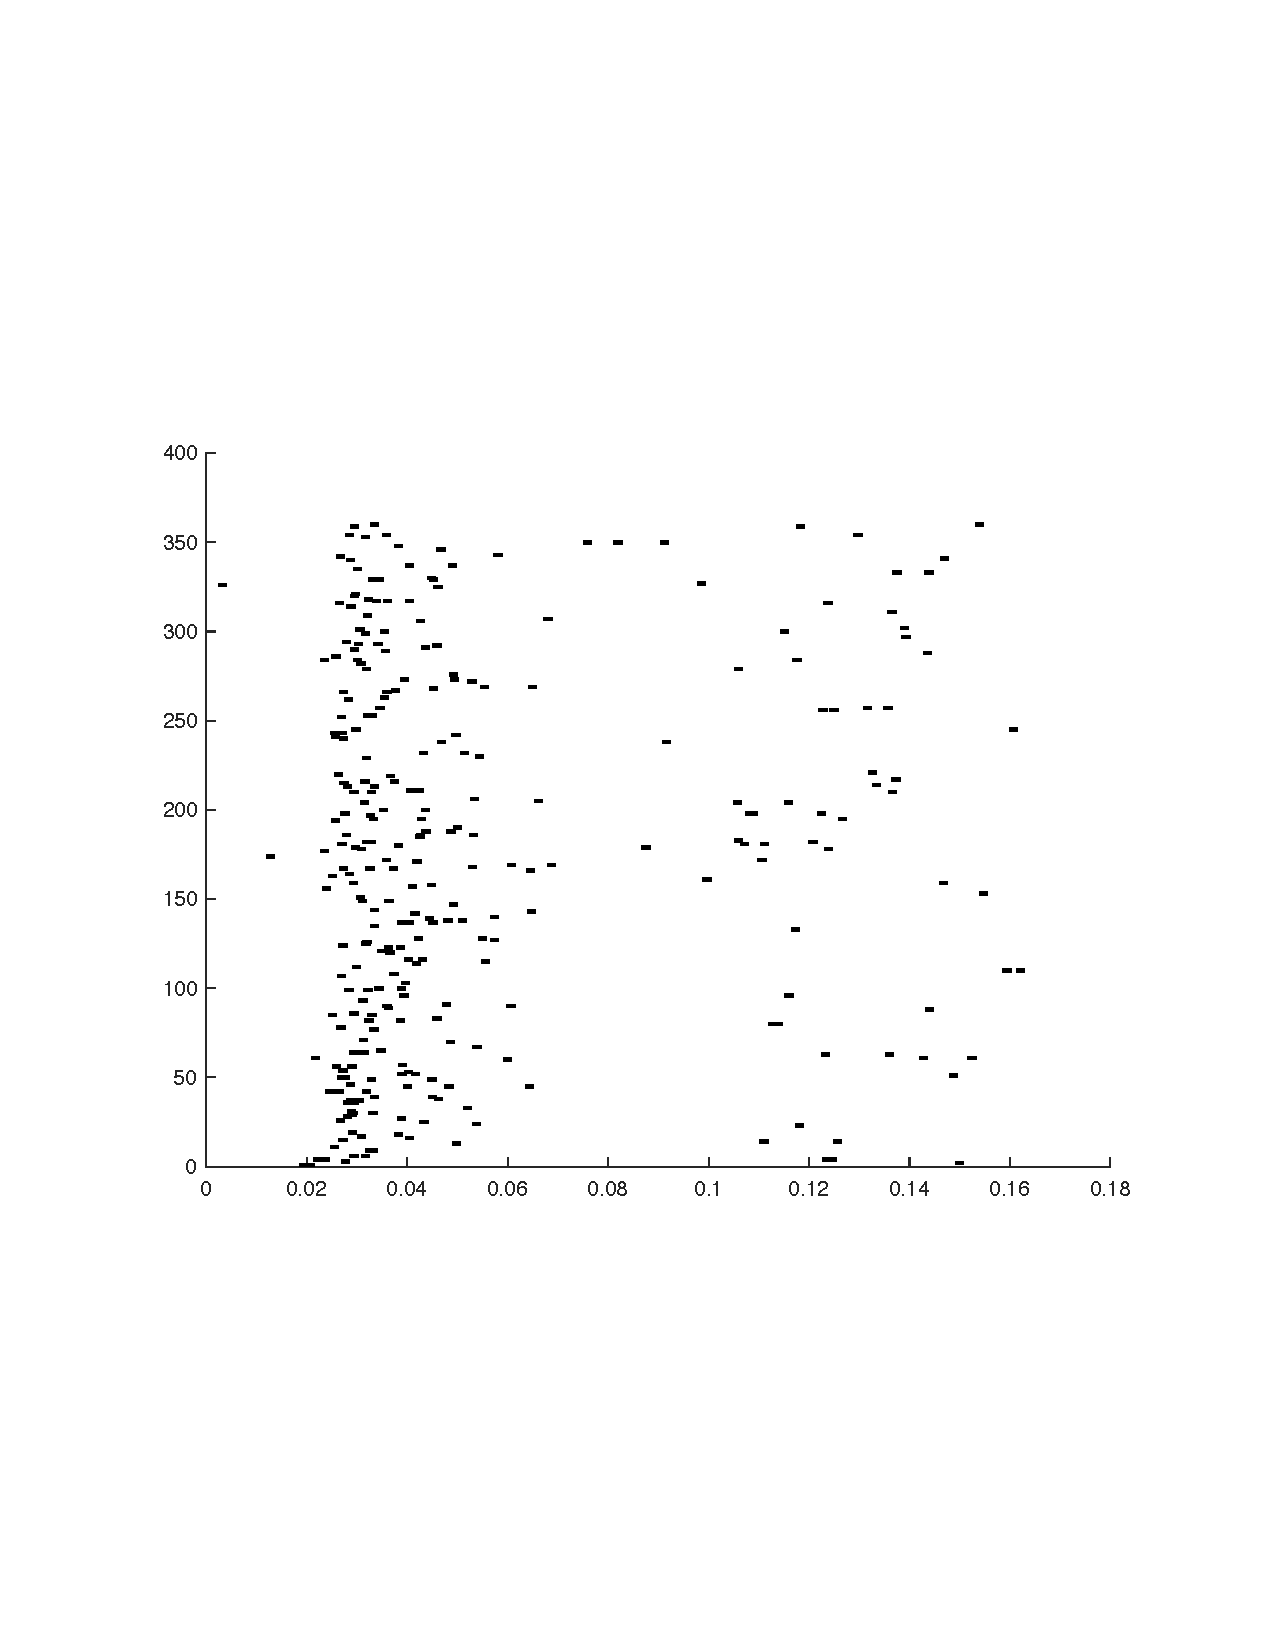
\includegraphics[width=0.6\linewidth]{problem1a.pdf}
    \caption{Raster plot as specified in the problem statement. Note that the neuron responds clearly to the stimulus, with a high density of spikes about 25 ms after it is played.}
    \label{fig:my_label}
\end{figure}

\subsection*{1b and 1c}

\begin{figure}[H]
    \centering
    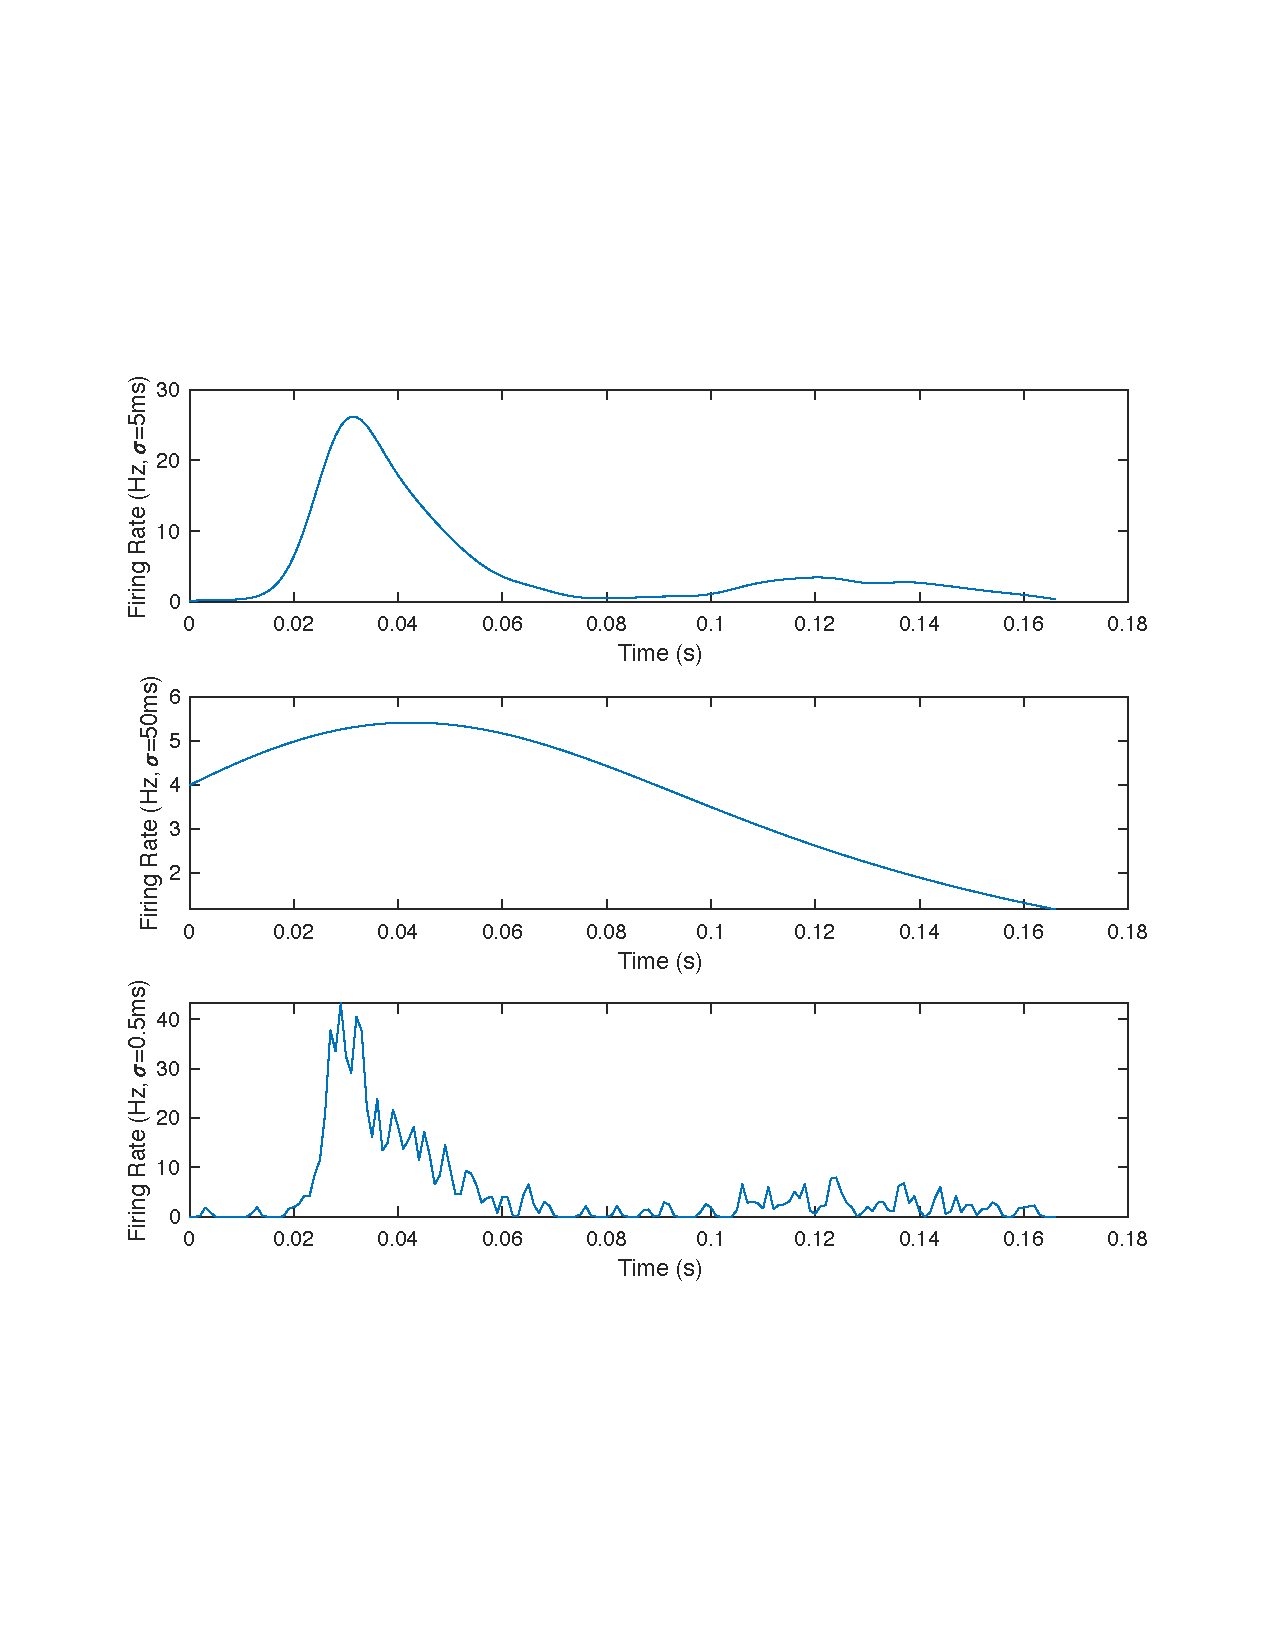
\includegraphics[width=0.8\linewidth]{problem1bc.pdf}
    \caption{Average firing rates using Gaussian smoothing kernels for $\sigma=5ms$, $\sigma=50ms$, and $\sigma=0.5ms$, respectively. From the second plot, it is clear that a larger standard deviation may not effectively capture more abrupt changes in the firing rate (note that the approximate firing rate is still relatively high at 0.08 seconds, while the true firing rate is essentially zero). Conversely, a smaller standard deviation may be too sensitive to the timing of individual spikes, oscillating wildly in a way that is unlikely to reflect the true operation of the neuron.}
    \label{fig:my_label}
\end{figure}

\subsection*{1d}

\begin{figure}[H]
    \centering
    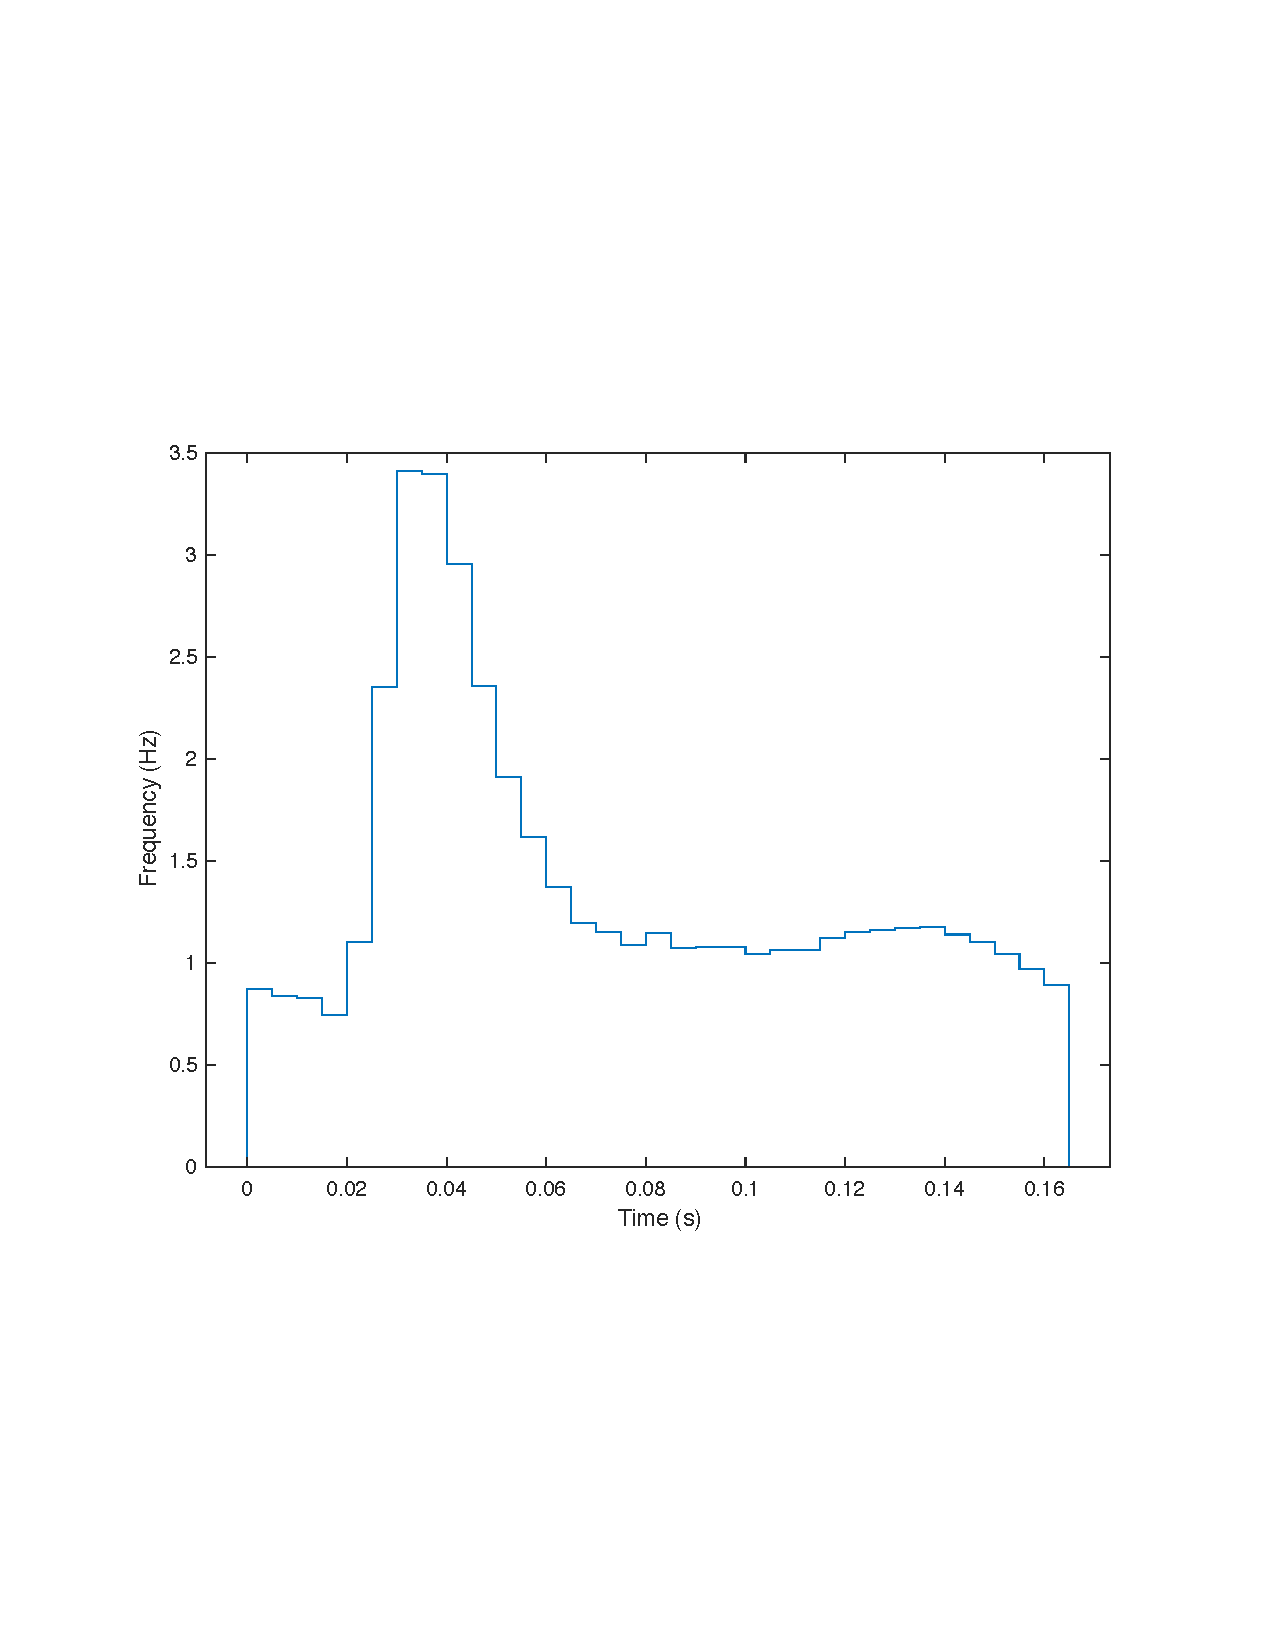
\includegraphics[width=0.5\linewidth]{problem1dExp.pdf}
    \caption{Grand average poststimulus time histogram for the experimental group.}
    \label{fig:my_label}
\end{figure}

\begin{figure}[H]
    \centering
    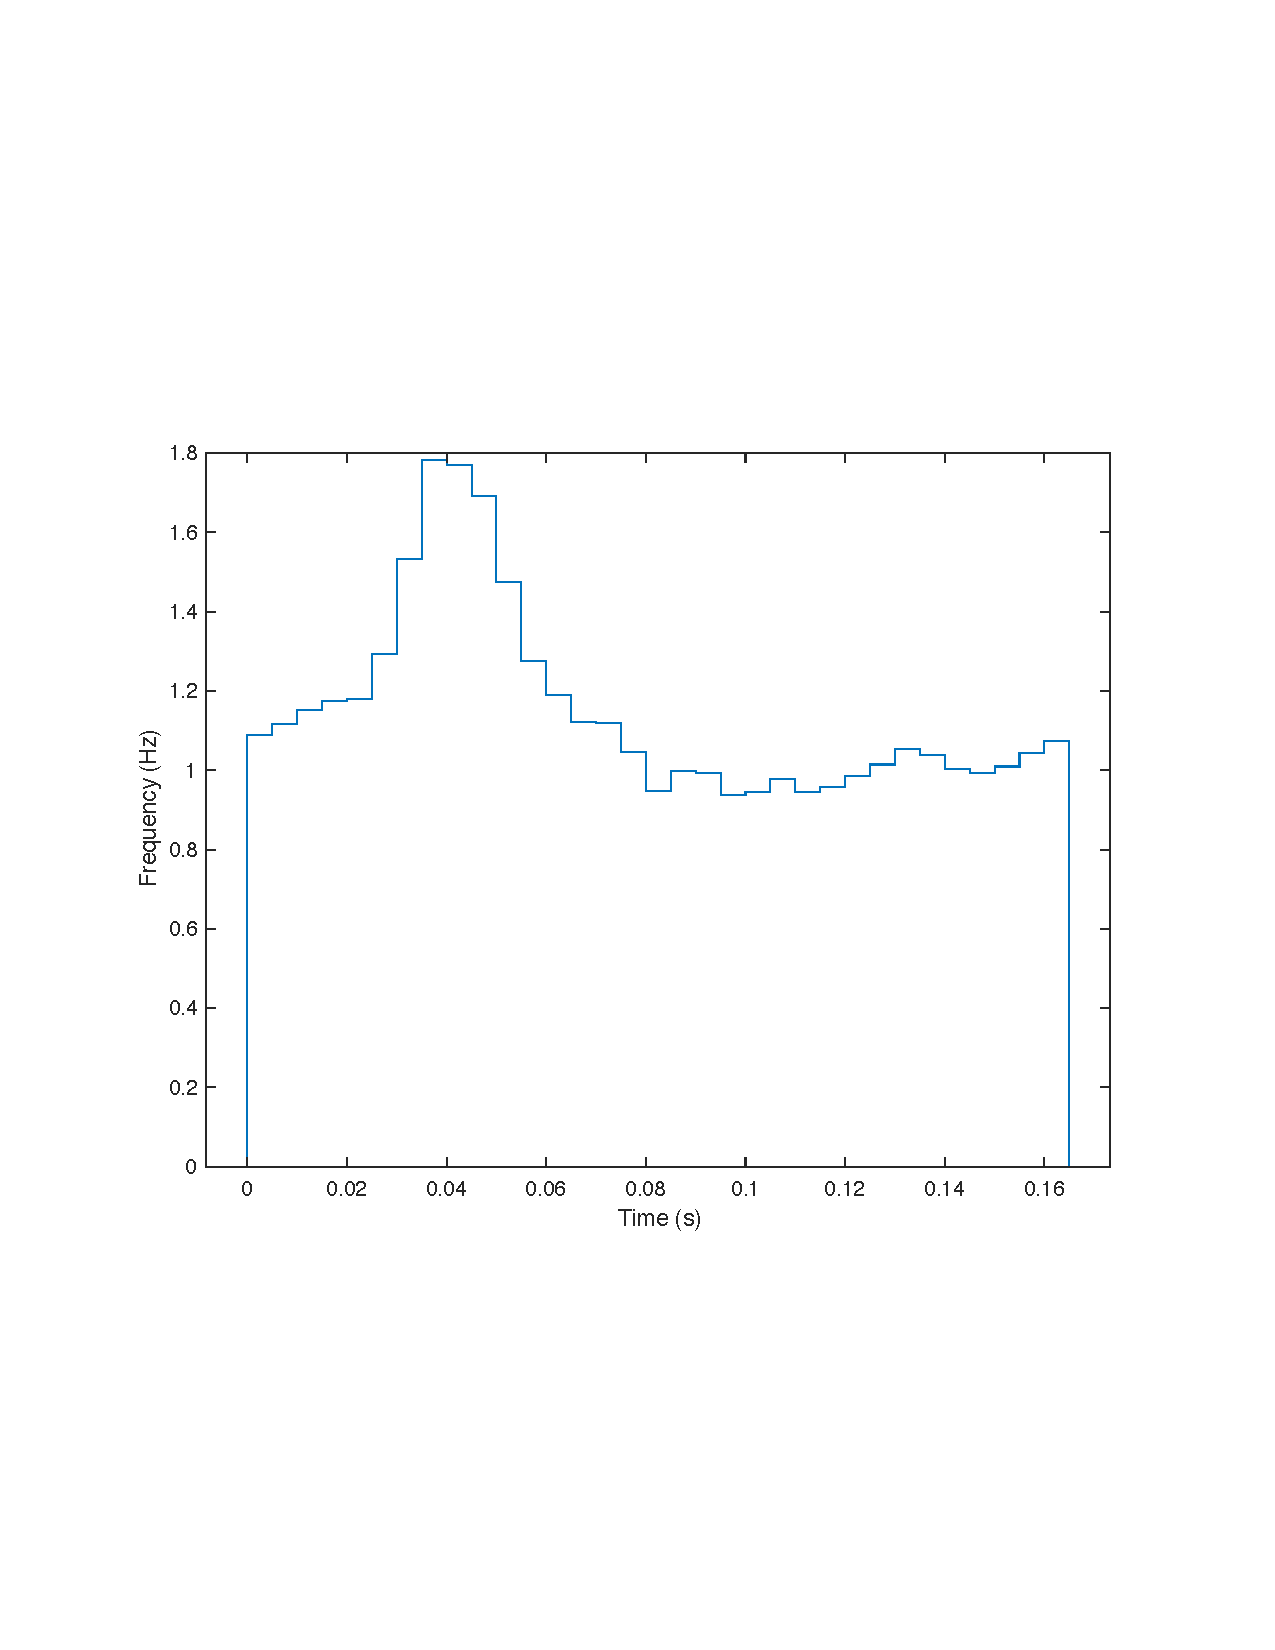
\includegraphics[width=0.5\linewidth]{problem1dControl.pdf}
    \caption{Grand average poststimulus time histogram for the control group.}
    \label{fig:my_label}
\end{figure}

\subsection*{1e}

The experimental group clearly demonstrates increased selectivity with respect to the stimulus, evidenced by a maximum poststimulus firing rate that is nearly double that of the control group. The response in the experimental group also exhibits heightened precision, with a more defined, narrower peak. After the initial peak response, the shape of the experimental group histogram resembles the single-unit firing rate response in the first plot of Figure 2, with a wide, smooth hump around 0.13 seconds; the control group does not exhibit this behavior. Moreover, in the experimental group, the average frequency after the initial peak response is higher than the average frequency before it. The opposite is true in the control group.

\subsection*{1f}

\begin{figure}[H]
    \centering
    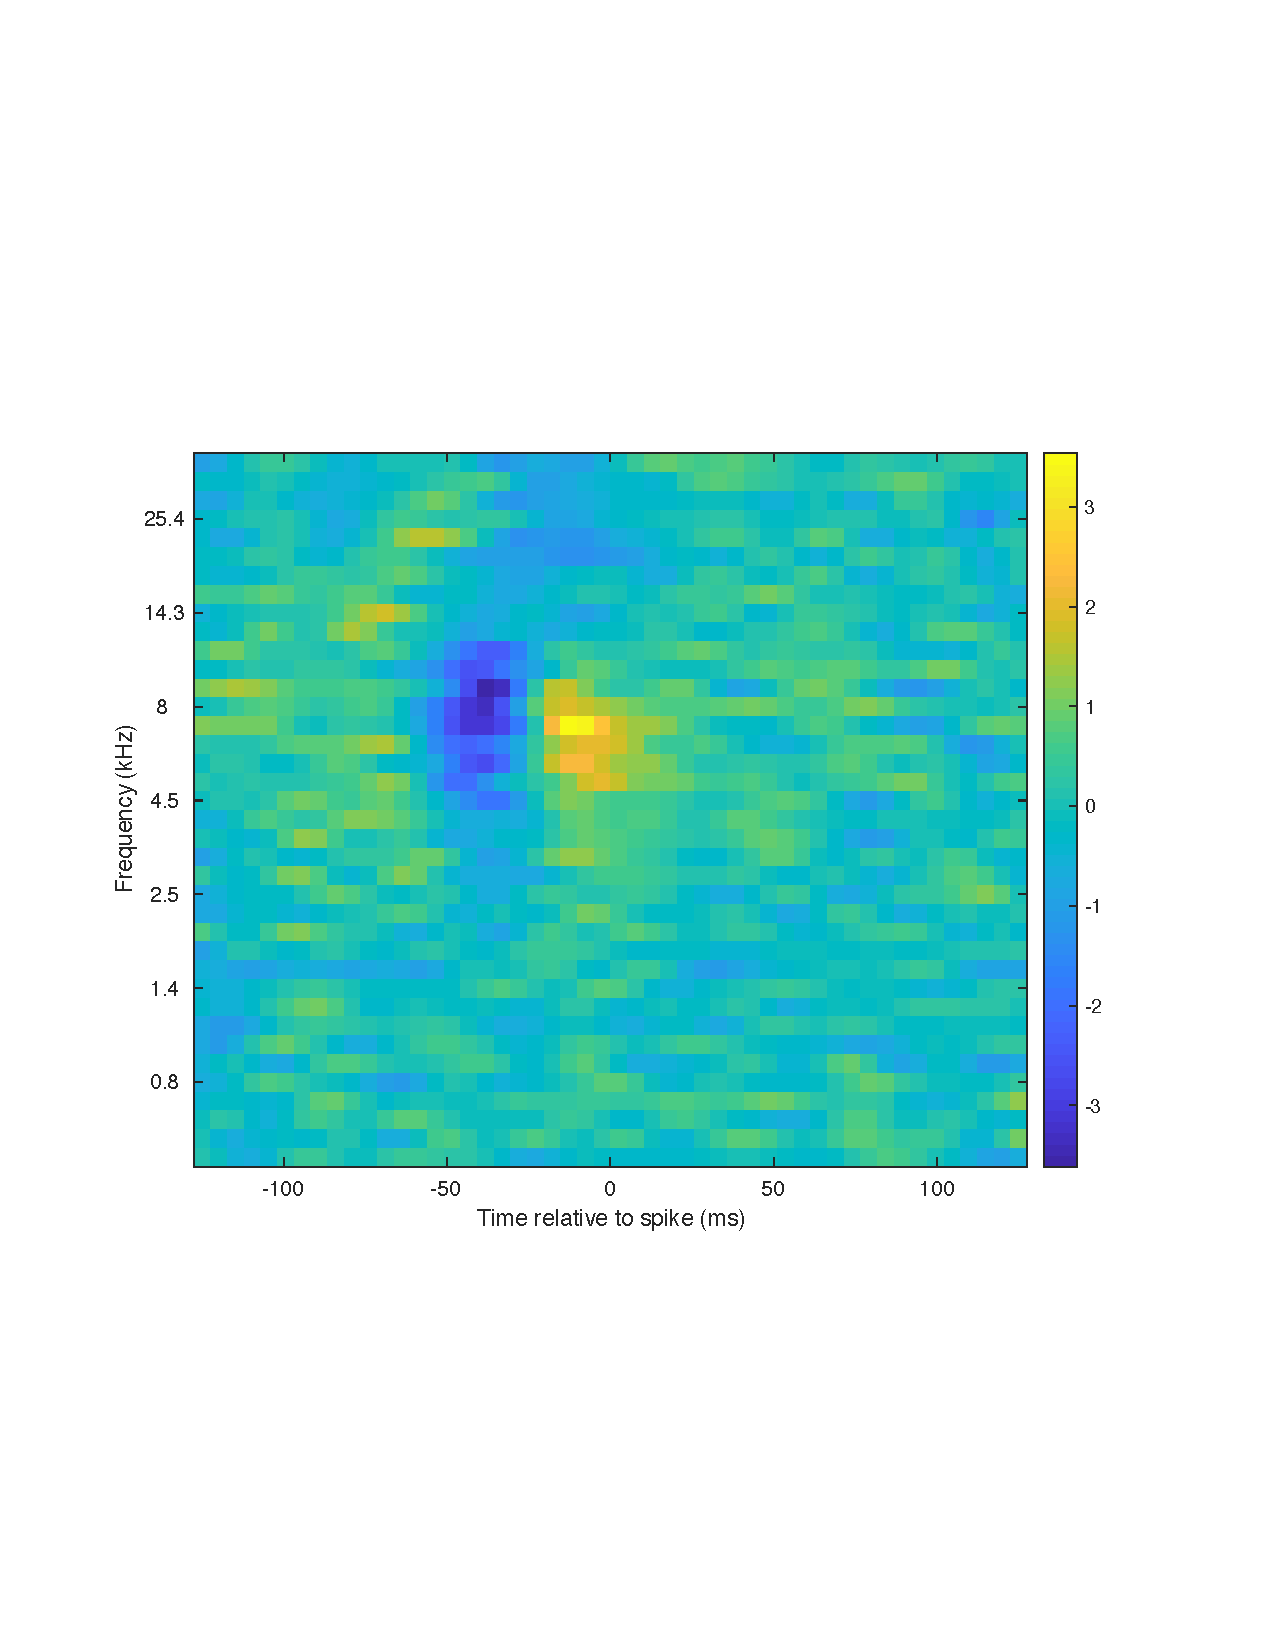
\includegraphics[width=0.8\linewidth]{problem1f.pdf}
    \caption{Spike-triggered average}
    \label{fig:my_label}
\end{figure}

\subsection*{1g}

The neuron is most selective to $\approx 7.1 kHZ$. We chose this value based on which frequency had the highest average intensity in the $25 ms$ preceding the spike.

\subsection*{1h}

The neuron's peak response would be higher to a brief tone pip. The STA shows that the neuron responds most strongly to a short period of absence of its preferred frequency (the dark blue patch) followed by a short period of high intensity of its preferred frequency (the bright yellow patch). The intensity of the neuron's preferred frequency is positive for about $25ms$ preceding the spike in the STA, suggesting that the tone pip to evoke the largest response would be about this length.

\subsection*{1i}

\begin{figure}[H]
    \centering
    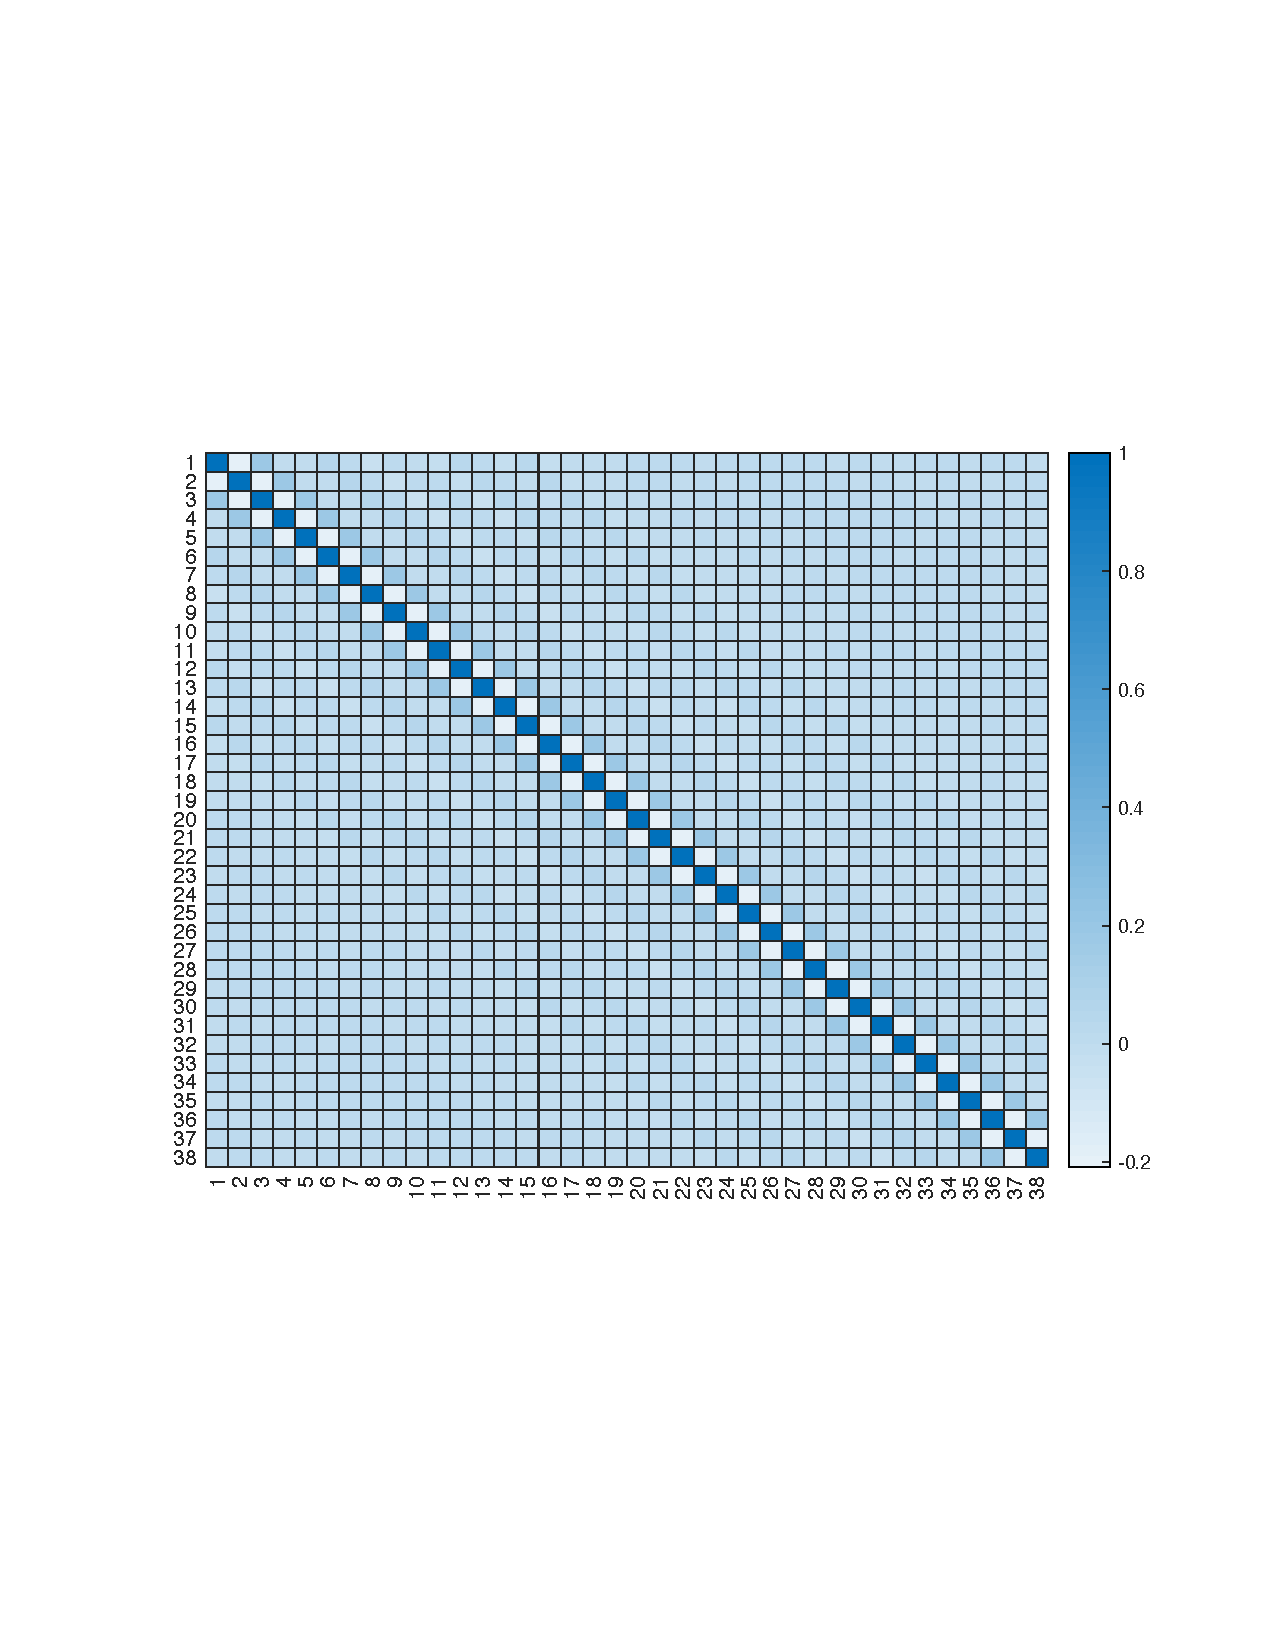
\includegraphics[width=0.8\linewidth]{problem1i.pdf}
    \caption{As exhibited above, the correlation matrix is almost precisely equal to the identity matrix. This is not $\texttt{stim\_spectrogram}*\texttt{stim\_spectrogram`}$ as suggested in the problem statement, but rather $\texttt{corrcov(cov(stim\_spectrogram`))}$, which is the true correlation matrix.}
    \label{fig:my_label}
\end{figure}

\section*{Problem 2}

\subsection*{2a}

\begin{figure}[H]
    \centering
    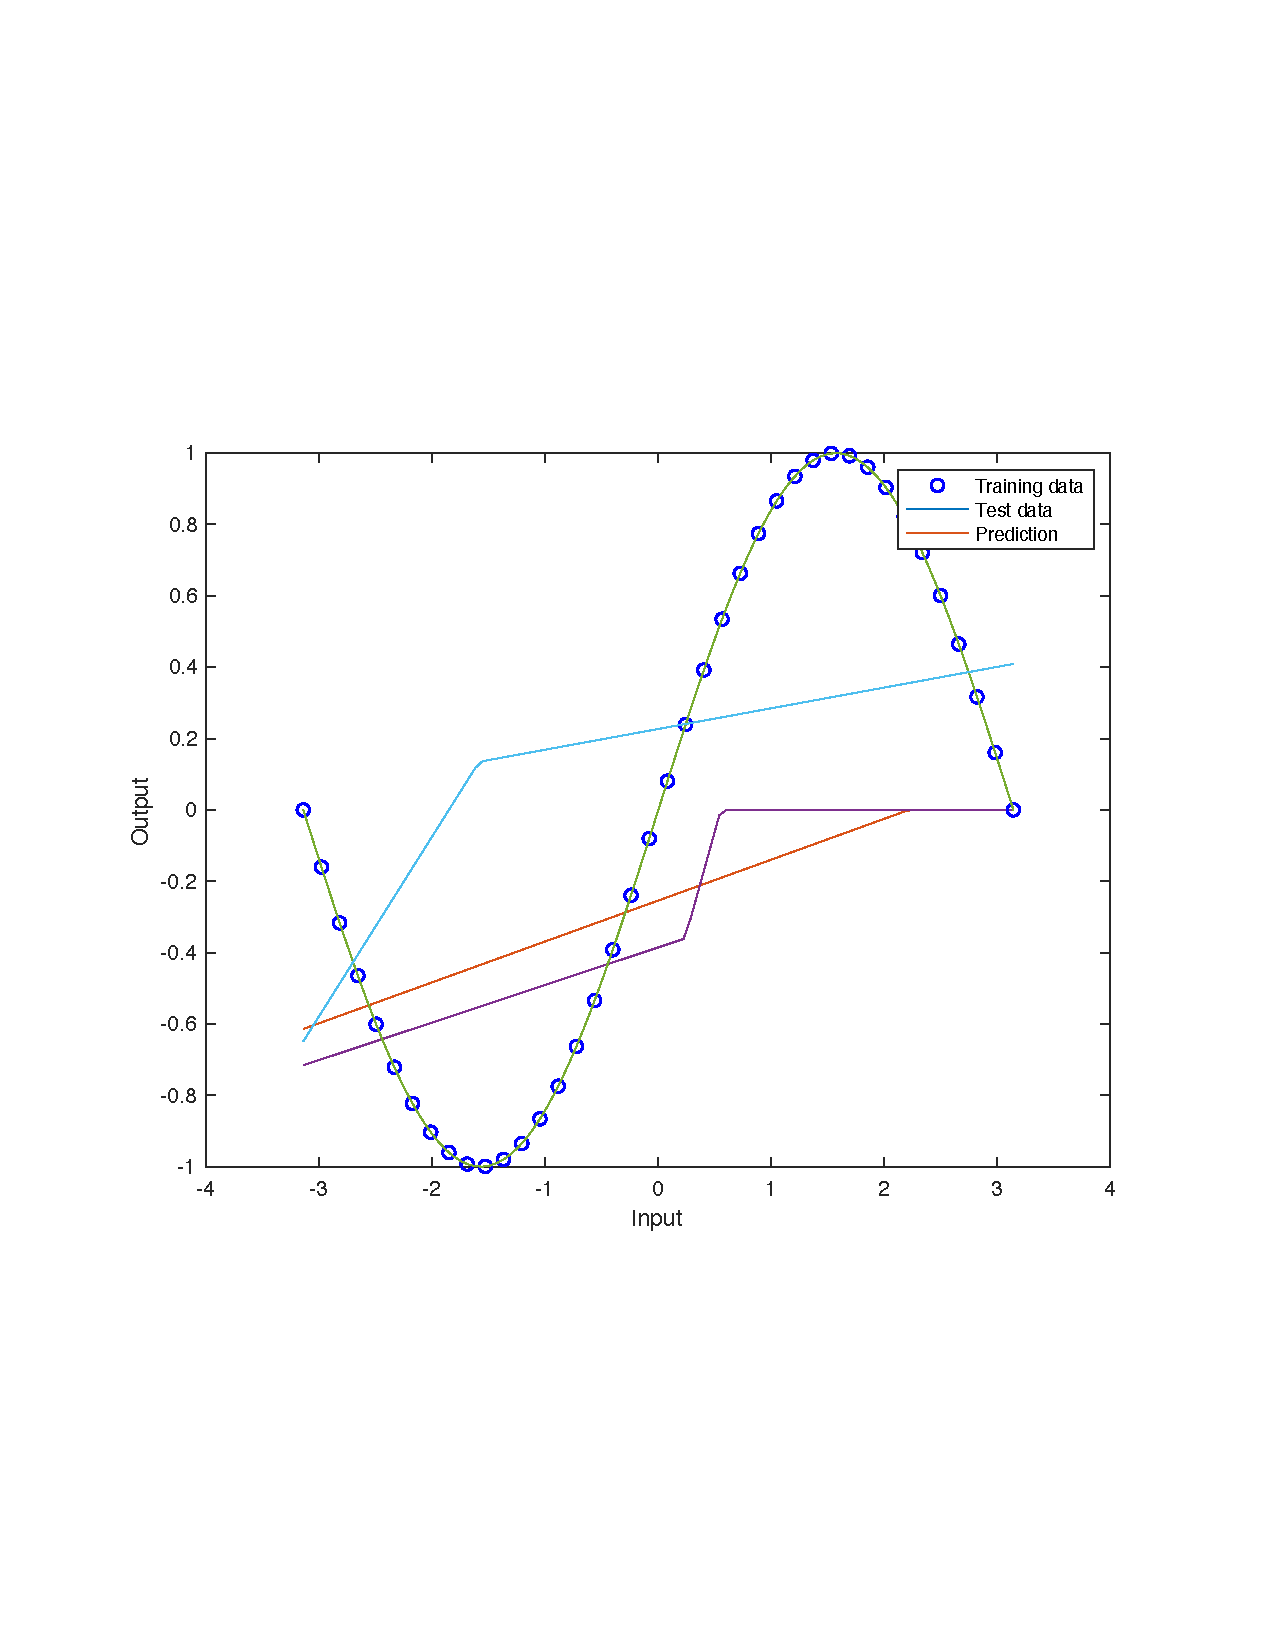
\includegraphics[width=0.6\linewidth]{problem2a2.pdf}
    \caption{Predictions on the test set overlaid on the true data for 3 different initializations of $J$ and $N_h=2$.}
    \label{fig:my_label}
\end{figure}

\begin{figure}[H]
    \centering
    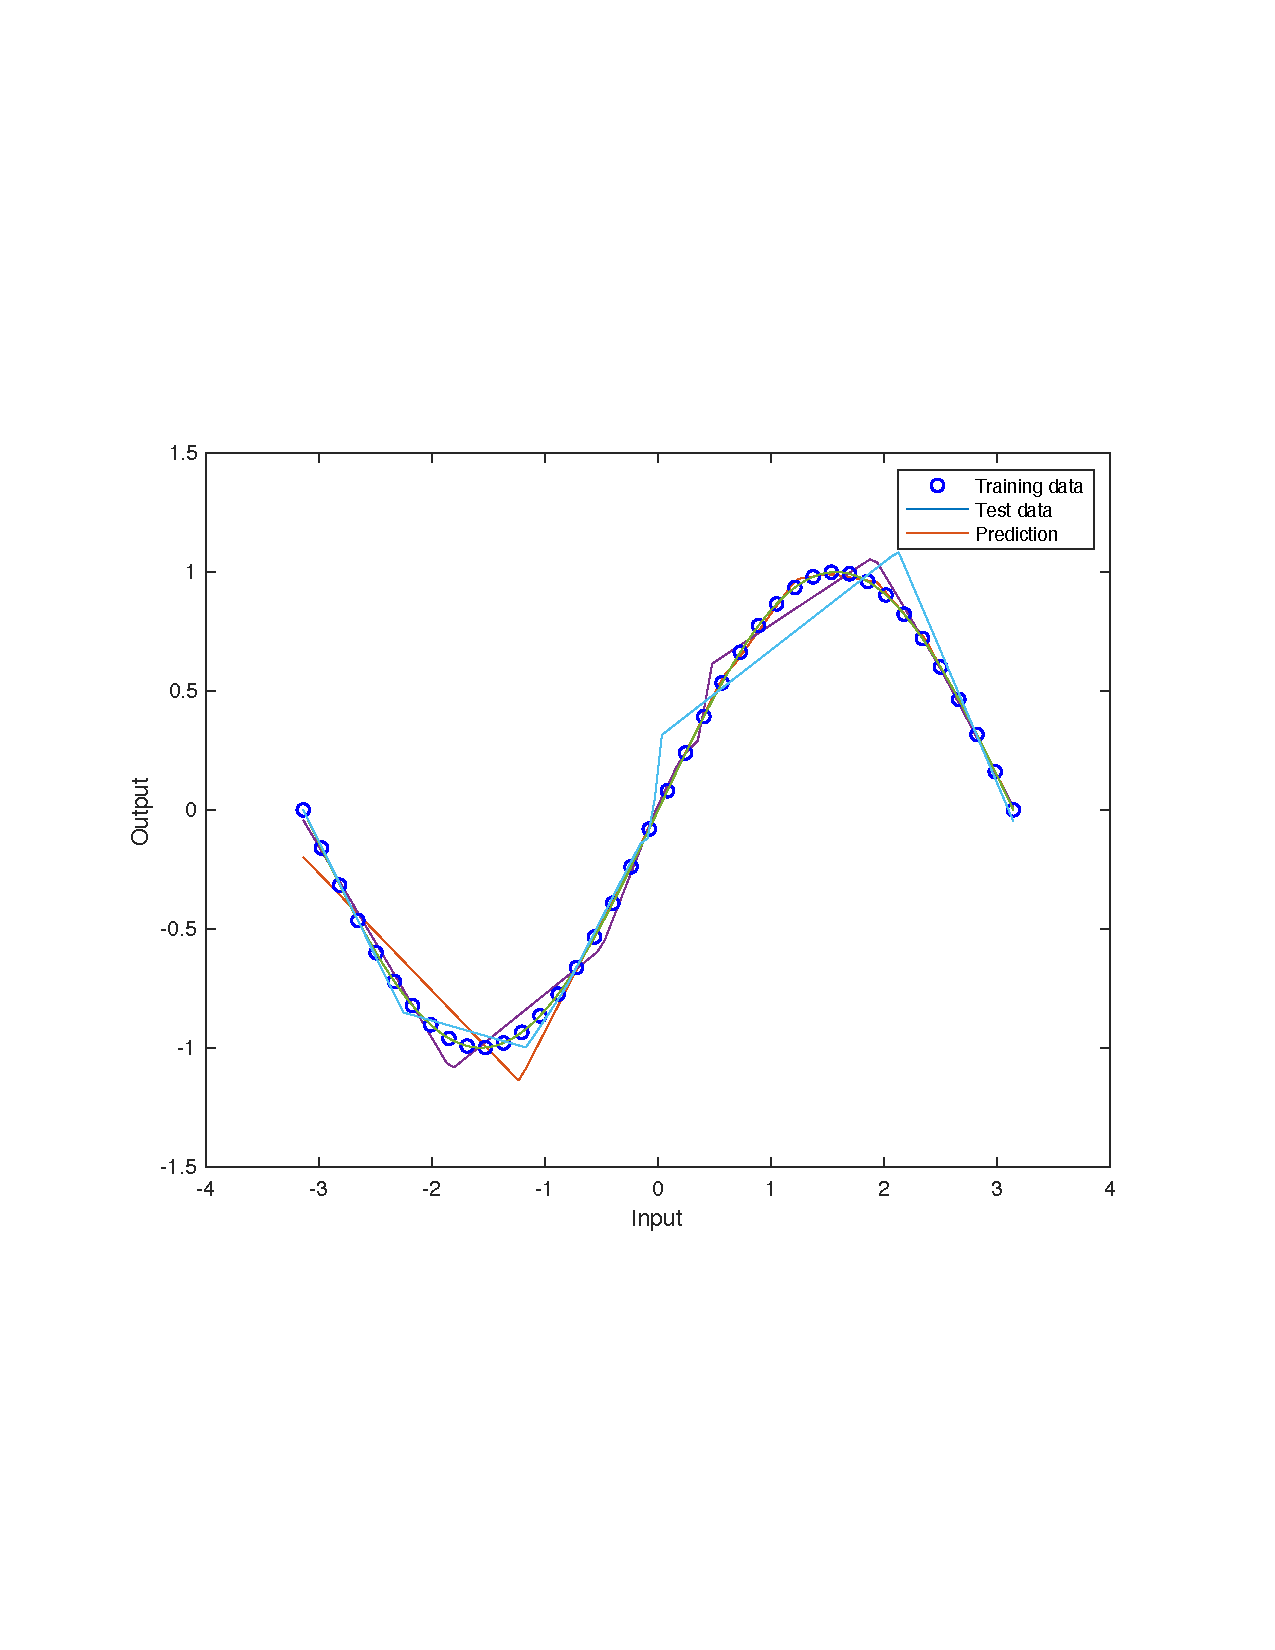
\includegraphics[width=0.6\linewidth]{problem2a10.pdf}
    \caption{Predictions on the test set overlaid on the true data for 3 different initializations of $J$ and $N_h=10$.}
    \label{fig:my_label}
\end{figure}

\begin{figure}[H]
    \centering
    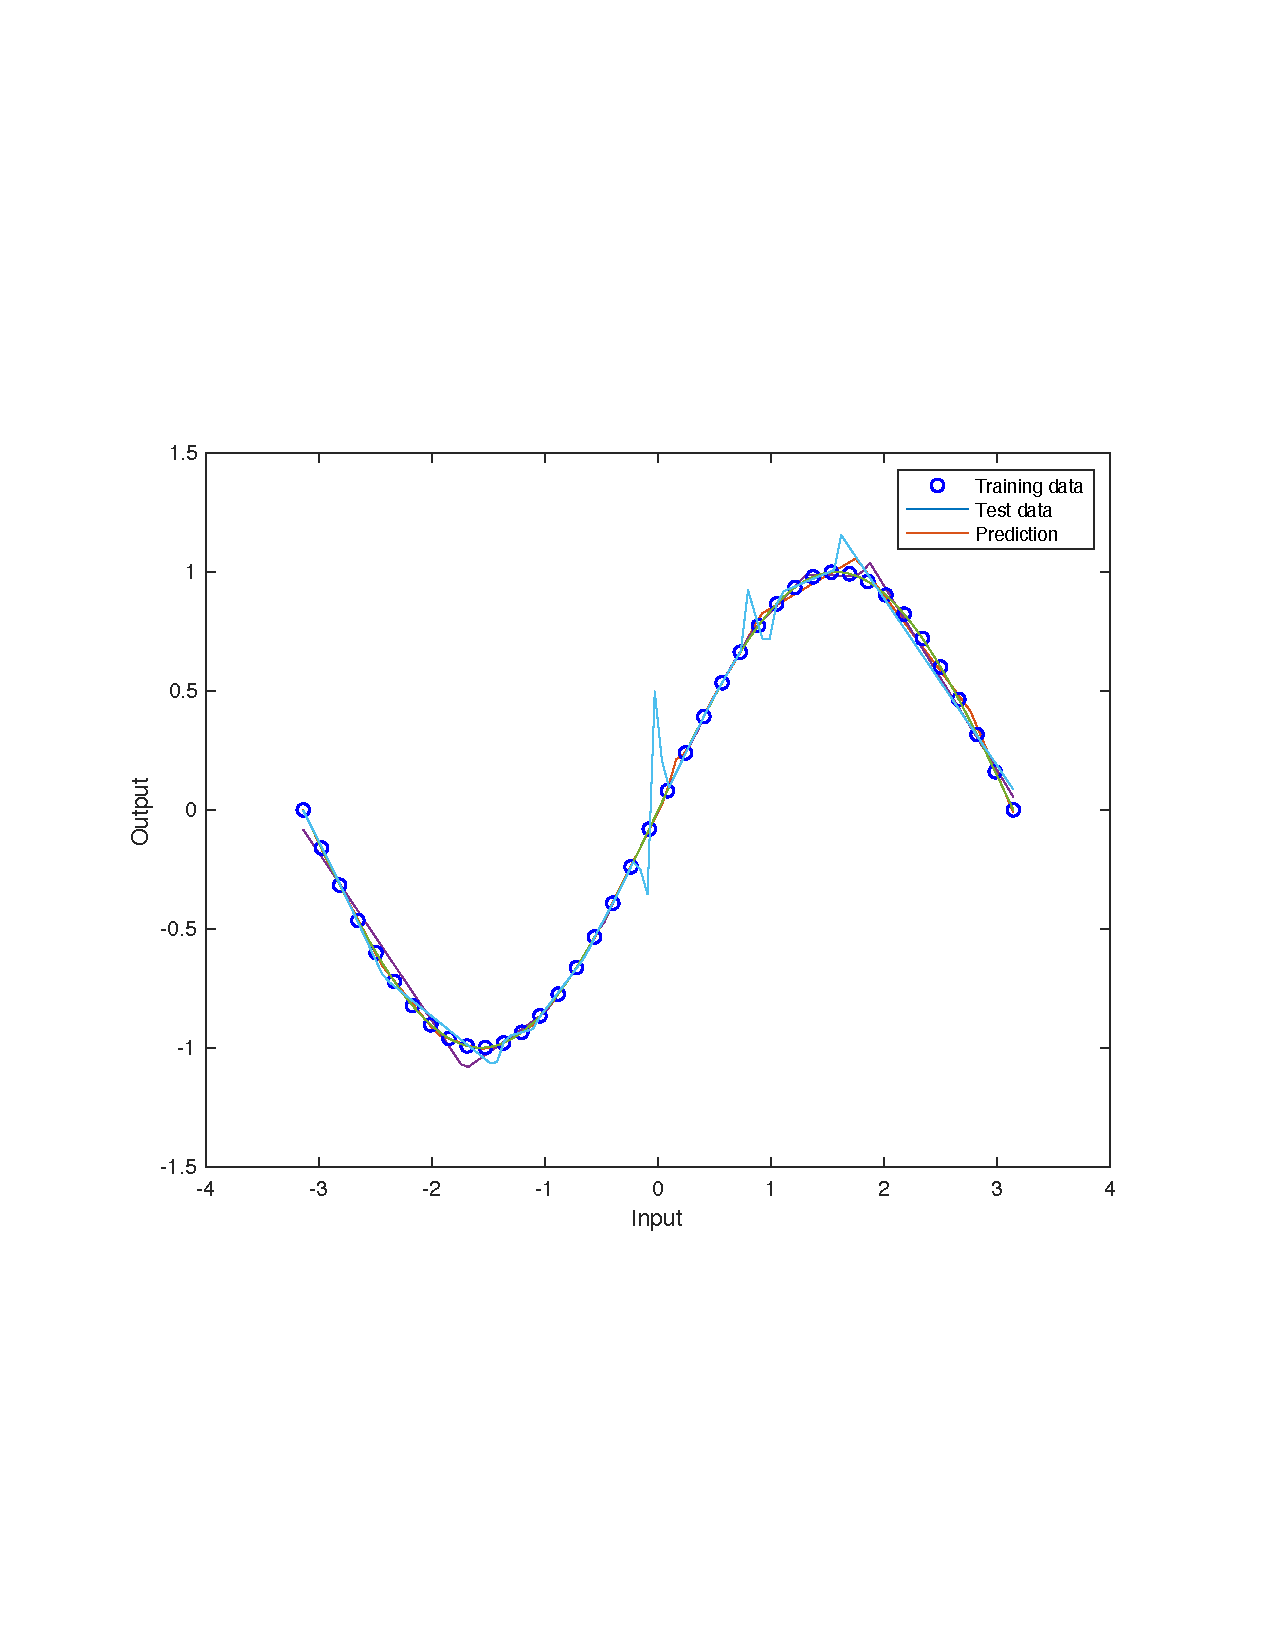
\includegraphics[width=0.6\linewidth]{problem2a26.pdf}
    \caption{Predictions on the test set overlaid on the true data for 3 different initializations of $J$ and $N_h=26$.}
    \label{fig:my_label}
\end{figure}

\subsection*{2b}

\begin{figure}[H]
    \centering
    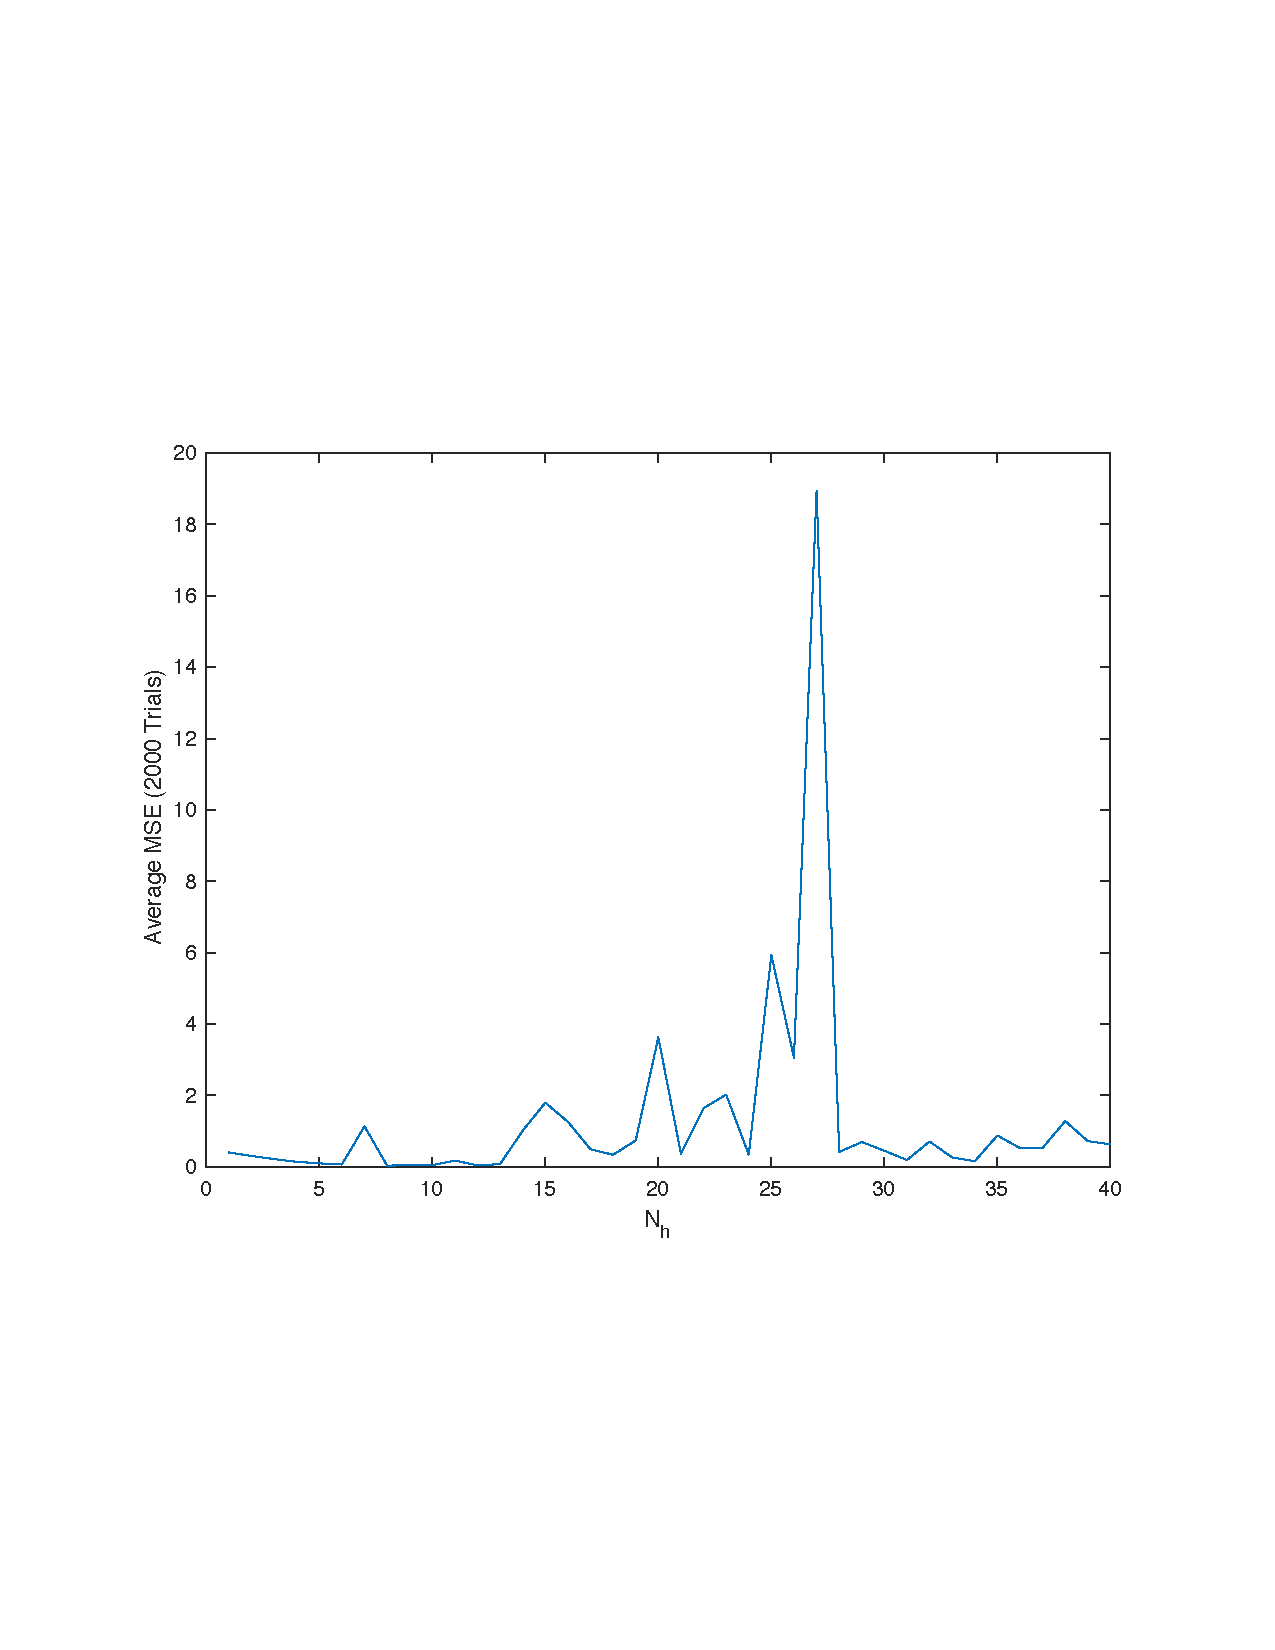
\includegraphics[width=0.55\linewidth]{problem2bNoReg.pdf}
    \caption{Average MSE (2000 trials) for $N_h=1$ to $N_h=40$, $\lambda=0$. Note that the distribution code computed total square error, and we modified it to compute MSE.}
    \label{fig:my_label}
\end{figure}

\begin{figure}[H]
    \centering
    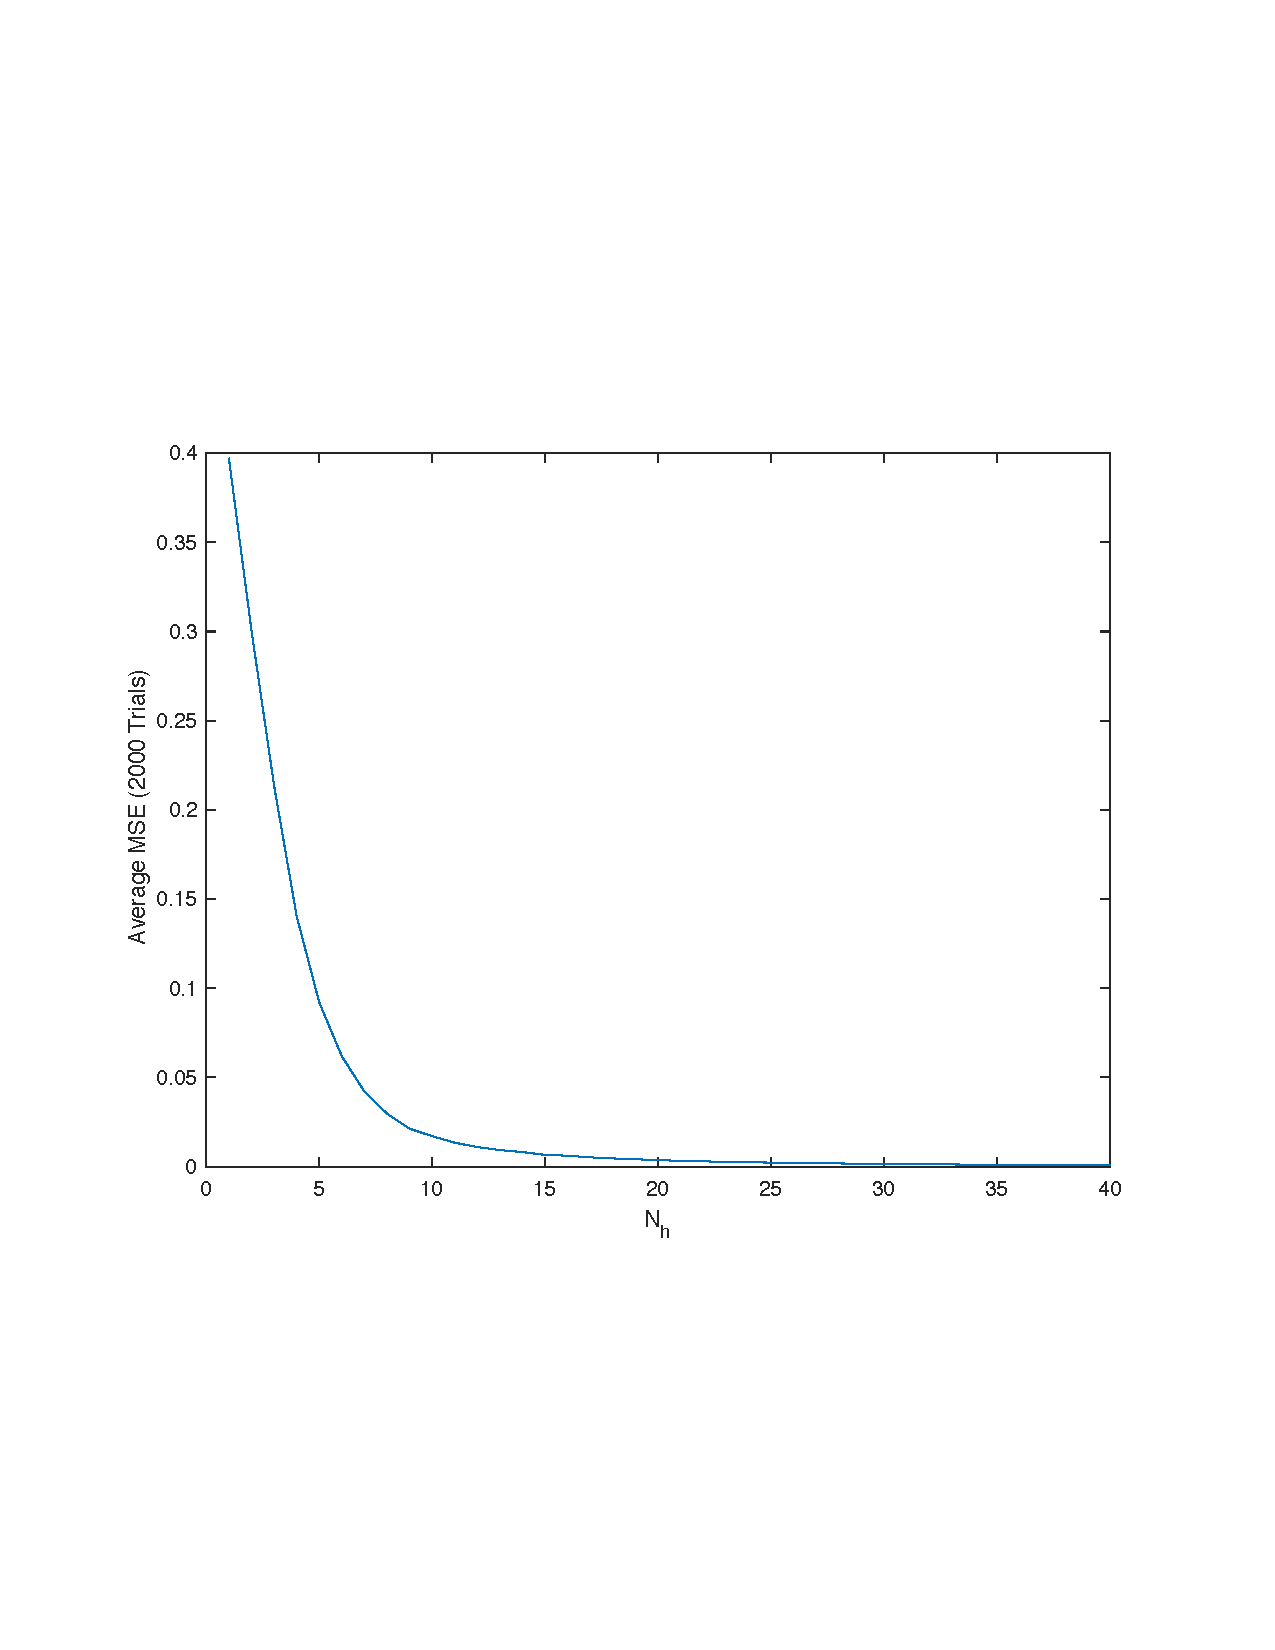
\includegraphics[width=0.55\linewidth]{problem2bReg1e-6.pdf}
    \caption{Average MSE (2000 trials) for $N_h=1$ to $N_h=40$, $\lambda=1e-6$. Note that the distribution code computed total square error, and we modified it to compute MSE.}
    \label{fig:my_label}
\end{figure}

The best model size depends on whether we use regularization or not. The odd spiking behavior in Figure 10 is a result of the randomness of $H$. When $\lambda=0$, $HH^\top$ is non-invertible with high probability and so the network exhibits unpredictable performance. Based on Figure 10, it would appear that the best model size is around 6. In Figure 11, we added a very small amount of regularization just to ensure that our solution could use a true inverse rather than a pseudoinverse. As expected, the regularization drastically lowers the variability of the performance of the network, with the average MSE monotonically decreasing as $N_h$ varies from 1 to 40. From Figure 11, we would determine that the best model size is $N_h=40$. Also as expected, a smaller model is less expressive and therefore cannot fully capture the variance in the data, as seen in the high test error for low values of $N_h$ in Figure 11. This model does not overfit for any value of $N_h$ between 1 and 40, as we can see by the nearly 0 test error for $N_h=40$. In general, though, a model that is too big may overfit. 

\end{document}
